% !TEX encoding = UTF-8 Unicode
%%%%%%%%%%%%%%%%%%%%%%%%%%%%%%%%%%%%%%%%%
% Beamer Presentation
% LaTeX Template
% Version 1.0 (10/11/12)
%
% This template has been downloaded from:
% http://www.LaTeXTemplates.com
%
% License:
% CC BY-NC-SA 3.0 (http://creativecommons.org/licenses/by-nc-sa/3.0/)
%
%%%%%%%%%%%%%%%%%%%%%%%%%%%%%%%%%%%%%%%%%

%----------------------------------------------------------------------------------------
%	PACKAGES AND THEMES
%----------------------------------------------------------------------------------------

\documentclass{beamer}

\mode<presentation> {

% The Beamer class comes with a number of default slide themes
% which change the colors and layouts of slides. Below this is a list
% of all the themes, uncomment each in turn to see what they look like.

%\usetheme{default}
%\usetheme{AnnArbor}
%\usetheme{Antibes}
%\usetheme{Bergen}
%\usetheme{Berkeley}
%\usetheme{Berlin}
%\usetheme{Boadilla}
%\usetheme{CambridgeUS}
%\usetheme{Copenhagen}
%\usetheme{Darmstadt}
%\usetheme{Dresden}
\usetheme{Frankfurt}
%\usetheme{Goettingen}
%\usetheme{Hannover}
%\usetheme{Ilmenau}
%\usetheme{JuanLesPins}
%\usetheme{Luebeck}
%\usetheme{Madrid}
%\usetheme{Malmoe}
%\usetheme{Marburg}
%\usetheme{Montpellier}
%\usetheme{PaloAlto}
%\usetheme{Pittsburgh}
%\usetheme{Rochester}
%\usetheme{Singapore}
%\usetheme{Szeged}
%\usetheme{Warsaw}

% As well as themes, the Beamer class has a number of color themes
% for any slide theme. Uncomment each of these in turn to see how it
% changes the colors of your current slide theme.

%\usecolortheme{albatross}
%\usecolortheme{beaver}
%\usecolortheme{beetle}
%\usecolortheme{crane}
%\usecolortheme{dolphin}
%\usecolortheme{dove}
%\usecolortheme{fly}
%\usecolortheme{lily}
%\usecolortheme{orchid}
%\usecolortheme{rose}
%\usecolortheme{seagull}
%\usecolortheme{seahorse}
%\usecolortheme{whale}
%\usecolortheme{wolverine}

%\setbeamertemplate{footline} % To remove the footer line in all slides uncomment this line
%\setbeamertemplate{footline}[page number] % To replace the footer line in all slides with a simple slide count uncomment this line

%\setbeamertemplate{navigation symbols}{} % To remove the navigation symbols from the bottom of all slides uncomment this line
}

\usepackage[portuguese]{babel}
\usepackage[utf8]{inputenc}
\usepackage{graphicx} % Allows including images
\usepackage{booktabs} % Allows the use of \toprule, \midrule and \bottomrule in tables
\usepackage{tikz}
\usepackage{stackengine}
\usepackage{hyperref}
\usepackage{subcaption}
\usepackage{float}
\usepackage{amsmath}

\usepackage{todonotes} % REMOVE LATER

%  NEW COMMANDS
\def\stackalignment{r}
\newcommand{\figcopyright}[4]
{
  \begin{figure}
    \stackunder{
      \includegraphics[width=0.75\linewidth]{#1}
    } {\raggedleft \tiny Fonte:\href{#2}{\textcopyright \ #3.}}
    \caption{#4}
  \end{figure}
}

\newcommand{\partfrac}[3] % Bugged function, must be called as \partfrac2
{
  \ensuremath{\dfrac{\partial{#2}}{\partial{#3}}}
}
%----------------------------------------------------------------------------------------
%	TITLE PAGE
%----------------------------------------------------------------------------------------

\title[Métodos Numéricos]{Simulação Numérica De Escoamentos Dispersos Utilizando Método De Elementos Finitos} % The short title appears at the bottom of every slide, the full title is only on the title page

\author{\textbf{Lucas Carvalho De Sousa} \\ Gustavo Rabello Dos Anjos} % Your name
\institute[UERJ] % Your institution as it will appear on the bottom of every slide, may be shorthand to save space
{
  Universidade do Estado do Rio de Janeiro \\ % Your institution for the title page
  \medskip
  \href{mailto:encarvlucas@hotmail.com}{\textit{encarvlucas@hotmail.com}} % Your email address
}
\date{7 de Janeiro de 2019} %\today Date, can be changed to a custom date

\titlegraphic{%
  \makebox[0.9\paperwidth]{%
    
\includegraphics[width=1.5cm,keepaspectratio]{figure/UERJ.png}%
    \hfill%
    
\includegraphics[height=1.5cm,keepaspectratio]{figure/fen-new.png}%
  }%
}

\begin{document}

\begin{frame}
  \titlepage % Print the title page as the first slide
\end{frame}

\begin{frame}
  \frametitle{Sumário} % Table of contents slide, comment this block out to remove it
  \tableofcontents % Throughout your presentation, if you choose to use \section{} and \subsection{} commands, these will automatically be printed on this slide as an overview of your presentation
\end{frame}

%----------------------------------------------------------------------------------------
%	PRESENTATION SLIDES
%----------------------------------------------------------------------------------------

%----------------------------------------------------------------------------------------------------------------------------------------------------
\section{Introdução} % Sections can be created in order to organize your presentation into discrete blocks, all sections and subsections are automatically printed in the table of contents as an overview of the talk
%----------------------------------------------------------------------------------------------------------------------------------------------------

\subsection{Motivação} % A subsection can be created just before a set of slides with a common theme to further break down your presentation into chunks
\begin{frame}
  \frametitle{Simulação de Escoamentos Multifásicos em Turbomáquinas}
  \figcopyright{figure/Washing_machine_agitator.jpg}
	       {https://commons.wikimedia.org/wiki/File:Washing_machine_agitator.JPG}
	       {BrokenSphere / Wikimedia Commons}
	       {Agitador de uma máquina de lavar.}
  
%   \figcopyright{figure/Aerial_view_of_the_Amazon_Rainforest.jpg}
% 	       {https://www.flickr.com/photos/lubasi/4909683043/}
% 	       {Lucía Barreiros}
% 	       {Rio Solimões - Amazônia, Brasil}
\end{frame}

% \begin{frame}
%   \frametitle{A Importância da Simulação de Escoamentos}
%   \figcopyright{figure/Cologne_Germany_Bundle-extractor-01.jpg}
% 	       {https://commons.wikimedia.org/wiki/File:Cologne_Germany_Bundle-extractor-01.jpg}
% 	       {CEphoto, Uwe Aranas}
% 	       {Interior de um trocador de calor - Colônia, Alemanha}
% \end{frame}

%----------------------------------------------------------------------------------------------------------------------------------------------------
\subsection{Escoamentos Dispersos}
\begin{frame}
  \frametitle{Escoamentos}
  \begin{figure}
    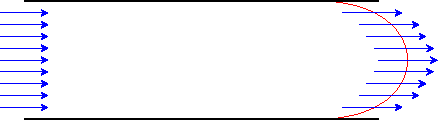
\includegraphics[width=\linewidth]{figure/developed_flow.pdf}
    \caption{Escoamento permanente desenvolvido.}
  \end{figure}
\end{frame}

\begin{frame}
  \frametitle{Escoamentos Multifásicos}
  \begin{figure}
    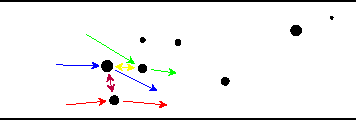
\includegraphics[width=\linewidth]{figure/particle_flow.pdf}
    \caption{Escoamento particulado.}
  \end{figure}
\end{frame}

%----------------------------------------------------------------------------------------------------------------------------------------------------
\section{Metodologia}
%----------------------------------------------------------------------------------------------------------------------------------------------------

\subsection{Malhas Computacionais}
\begin{frame}
  \frametitle{Discretização}
  
  \begin{figure}
    \title{Soluções da pressão}
    \begin{minipage}[t]{.49\textwidth}
      \centering
      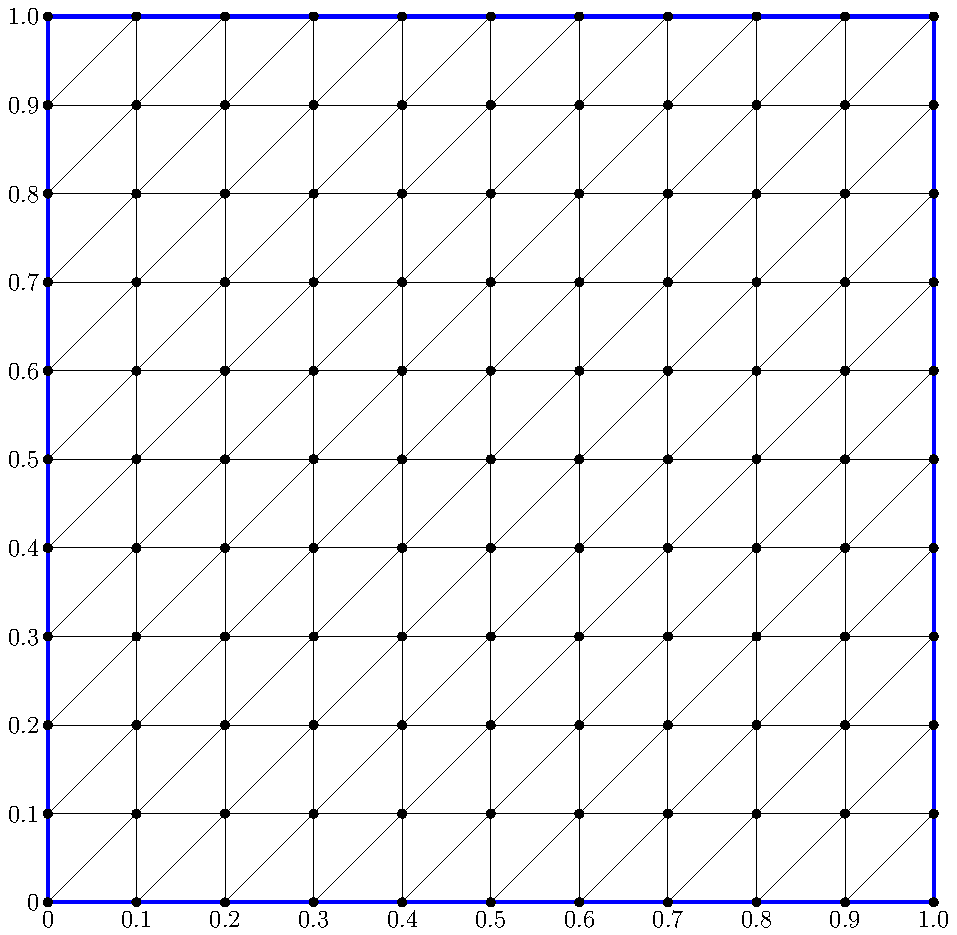
\includegraphics[height=0.95\linewidth]{figure/structured_mesh.pdf}
      \captionof{figure}{Malha estruturada.}
    \end{minipage}
    \hfill
    \begin{minipage}[t]{.49\textwidth}
      \centering
      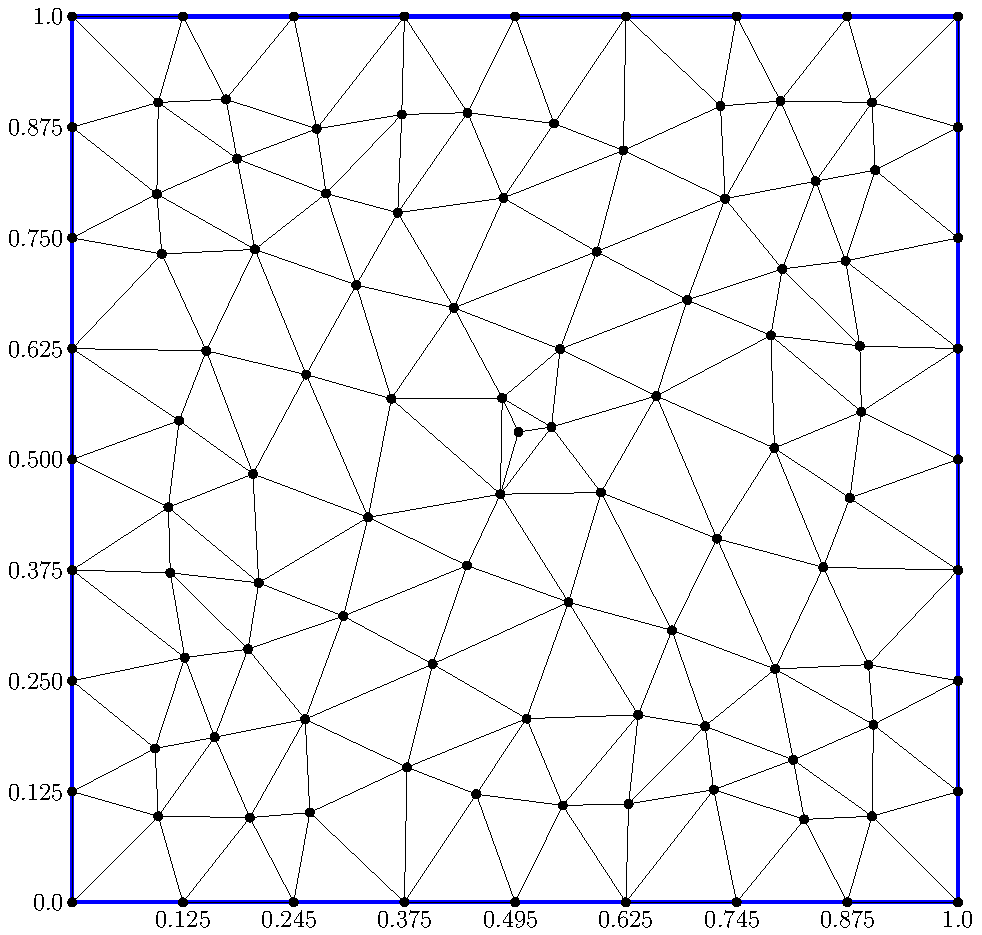
\includegraphics[height=0.95\linewidth]{figure/unstructured_mesh.pdf}
      \captionof{figure}{Malha não estruturada.}
    \end{minipage}
  \end{figure}
\end{frame}

%----------------------------------------------------------------------------------------------------------------------------------------------------
\subsection{Sistema de Equações}
\begin{frame}
  \frametitle{Modelo Matemático}
  \begin{minipage}{.48\textwidth}
    \begin{block}{Equação de Vorticidade}
      \centering
      $\partfrac2{\omega_z}{t} + \vec{v}.\nabla\omega_z = \nu \nabla^2 \omega_z$
    \end{block}

    \begin{block}{Equação de Corrente}
      \centering
      $\nabla^2 \psi = -\omega_z$
    \end{block}
    
    \begin{block}{Equação BBO (\it{Basset–Boussinesq–Oseen})}
      \centering
      $\sum \vec{F}_p = \vec{F}_{drag} + \vec{F}_{grav} + \vec{F}_{etc}$
    \end{block}
  \end{minipage}
  \hfill
  \begin{minipage}{.48\textwidth}
    \begin{block}{Equações Auxiliares}
      \vspace*{-\baselineskip}\setlength\belowdisplayshortskip{0pt} % Fix display bug, empty header space
      \centering
      \begin{align*}
	\partfrac2{\psi}{y} &= v_x \\
	\partfrac2{\psi}{x} &= -v_y \\
	\omega_z &= \partfrac2{v_x}{y} - \partfrac2{v_y}{x} 
      \end{align*}
    \end{block}
  \end{minipage}
  
\end{frame}

\begin{frame}
  \frametitle{Modelo Matemático}
  \begin{block}{Força de Arrasto (\it{Stoakes})}
    \centering
    $\vec{F}_{drag} = 3 \pi \mu d_p (\vec{v} - \vec{v}_p)$
  \end{block}
  \begin{block}{Força Gravitacional}
    \centering
    $\vec{F}_{grav} = \tfrac{\pi}{6} d_p \rho_p \vec{g}$
  \end{block}
  
  Onde: $\omega_z$ é o campo de vorticidade, $\psi$ é o campo de correntes, $\vec{v}$ é o campo vetorial de velocidades, 
  $\mu$ é a viscosidade dinâmica, $\nu$ é a viscosidade cinemática sobre o domínio da malha.
  E as variáveis $d_p$ são o diâmetro, $\rho_p$ é a densidade e $\vec{F}_p$ é a força resultante de uma partícula.
\end{frame}

%----------------------------------------------------------------------------------------------------------------------------------------------------
\subsection{Equações Matriciais}
\begin{frame}
  \frametitle{Matrizes dos Elementos Triangulares}
  \begin{minipage}{.25\textwidth}
    \centering
    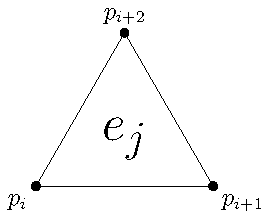
\includegraphics[width=0.95\linewidth]{figure/element.pdf}
  \end{minipage}
  \hfill
  \begin{minipage}{.7\textwidth}
    \begin{block}{Coeficientes de Forma}
      \vspace*{-\baselineskip}\setlength\belowdisplayshortskip{0pt} % Fix display bug, empty header space
      \centering
      \begin{equation*}
      \mathbf{B} \left\{
	\begin{align*}
	  &b_i = y_j - y_k \\
	  &b_j = y_k - y_i \\
	  &b_k = y_i - y_j
	\end{align*} \right.\qquad
      \mathbf{C} \left\{
	\begin{align*}
	  &c_i = x_k - x_j \\
	  &c_j = x_i - x_k \\
	  &c_k = x_j - x_i
	\end{align*} \right.
      \end{equation*}
    \end{block}
  \end{minipage}
  
  \begin{minipage}[t]{.45\textwidth}
    \centering
    \begin{block}{Matriz de Gradiente (eixo x)}
      $\mathbf{G}_x = \frac{1}{6}
	\begin{bmatrix}
	  b_i & b_j & b_k \\
	  b_i & b_j & b_k \\
	  b_i & b_j & b_k
	\end{bmatrix}$
    \end{block}
  \end{minipage}
  \hfill
  \begin{minipage}[t]{.45\textwidth}
    \centering
    \begin{block}{Matriz de Gradiente (eixo y)}
      $\mathbf{G}_y = \frac{1}{4A}
	\begin{bmatrix}
	  c_i & c_j & c_k \\
	  c_i & c_j & c_k \\
	  c_i & c_j & c_k
	\end{bmatrix}$
    \end{block}
  \end{minipage}
  
  \begin{minipage}[t]{.63\textwidth}
    \centering
    \begin{block}{Matriz de Rigidez}
      \footnotesize
      $\mathbf{K} = \frac{1}{4A}
	\begin{bmatrix}
	  b_i^2 + c_i^2 & b_i b_j + c_i c_j & b_i b_k + c_i c_k \\
	  b_j b_i + c_j c_i & b_j^2 + c_j^2 & b_j b_k + c_j c_k \\
	  b_k b_i + c_k c_i & b_k b_j + c_k c_j & b_k^2 + c_k^2
	\end{bmatrix}$
    \end{block}
  \end{minipage}
  \hfill
  \begin{minipage}[t]{.33\textwidth}
    \centering
    \begin{block}{Matriz de Massa}
      $\mathbf{M} = \frac{A}{12}
	\begin{bmatrix}
	  2 & 1 & 1   \\
	  1 & 2 & 1   \\
	  1 & 1 & 2  
	\end{bmatrix}$
    \end{block}
  \end{minipage}
\end{frame}

\begin{frame}
  \frametitle{Equações Matriciais}
  \begin{minipage}{.63\textwidth}
    \centering
    \begin{block}{Vorticidade}
      \centering
      $\bigg(\dfrac{\mathbf{M}}{\Delta t} + \nu \mathbf{K} + \mathbf{v.G} \bigg)\omega_z^{n+1} = \dfrac{\mathbf{M}}{\Delta t} \omega_z^n$
    \end{block}
    
    \begin{block}{Corrente}
      \centering
      $\mathbf{K} \psi = \mathbf{M} \omega_z$
    \end{block}
  \end{minipage}
  \hfill
  \begin{minipage}{.33\textwidth}
    \centering
    \begin{block}{Auxiliares}
      \vspace*{-\baselineskip}\setlength\belowdisplayshortskip{0pt} % Fix display bug, empty header space
      \centering
      \begin{align*}
	\mathbf{M} v_x &= \mathbf{G}_y \psi \\
	\mathbf{M} v_y &=-\mathbf{G}_x \psi \\
	\mathbf{M} \omega_z &= \mathbf{G}_x v_y - \mathbf{G}_y v_x
      \end{align*}
    \end{block}
  \end{minipage}
  
  \ \\
  As demais equações de força são calculadas para cada partícula individulamente.
\end{frame}

%----------------------------------------------------------------------------------------------------------------------------------------------------
\section{Resultados Preliminares}
%----------------------------------------------------------------------------------------------------------------------------------------------------

\begin{frame}
  \frametitle{Problema Físico}
  \todo[inline]{Inserir quais resultados?}
\end{frame}

%----------------------------------------------------------------------------------------------------------------------------------------------------
\section{Cronograma Futuro}
%----------------------------------------------------------------------------------------------------------------------------------------------------

\begin{frame}
  \frametitle{Atividades Concluídas e Previsão}
  \begin{figure}
    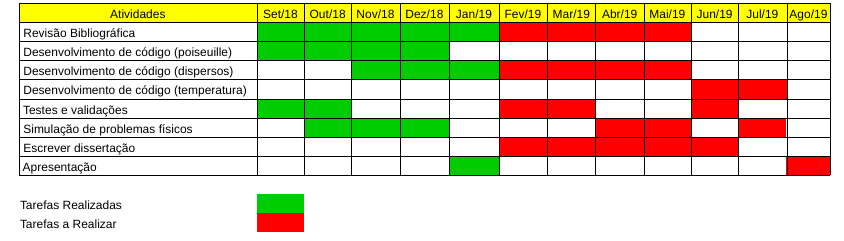
\includegraphics[width=\linewidth]{figure/Cronograma.png}
    \caption{Cronograma previsto atualizado.}
  \end{figure}
\end{frame}


%----------------------------------------------------------------------------------------------------------------------------------------------------
% Bibliografia
%----------------------------------------------------------------------------------------------------------------------------------------------------

% \begin{frame}
%   \frametitle{Bibliografia}
%   \footnotesize{
%     \todo[inline]{Fazer bibliografia}
%     \begin{thebibliography}{99} % Beamer does not support BibTeX so references must be inserted manually as below
% 
%       \bibitem[biezuner]{p1} R.J. Biezuner (2007)
%       \newblock Métodos Numéricos para Equações Parciais Elípticas
%       \newblock \emph{Notas de Aula}
% 
%       \bibitem[fortuna]{p1} A.O. Fortuna (2000)
%       \newblock Técnicas Computacionais para Dinâmica dos Fluidos: Conceitos Básicos e Aplicações
%       \newblock \emph{Edusp}
% 
%       \bibitem[leveque]{p1} R.J. LeVeque (2007)
%       \newblock Finite Difference Methods for Ordinary and Partial Differential Equations. Steady-State and Time-Dependant Problems
%       \newblock \emph{SIAM}
% 
%       \bibitem[biezuner]{p1} J.R. Rodrigues (2015)
%       \newblock Introdução à Simulação de Reservatórios Petrolíferos
%       \newblock \emph{Programa de Verão LNCC}
%     \end{thebibliography}
%   }
% \end{frame}

%----------------------------------------------------------------------------------------------------------------------------------------------------
% Agradecimentos
%----------------------------------------------------------------------------------------------------------------------------------------------------

\begin{frame}
  \frametitle{Agradecimentos}
  \centering
  \begin{tikzpicture}
    \node[inner sep=0cm] (gesar) at (0,0){
      
\includegraphics[width=0.2\textwidth]{figure/gesar-logo-new.png}};
    \node[inner sep=0cm] (uerj) at (4,0){
      
\includegraphics[width=0.2\textwidth]{figure/UERJ.png}};
    \node[inner sep=0cm] (fen) at (8,0){
      
\includegraphics[width=0.2\textwidth]{figure/fen-new.png}};
  \end{tikzpicture}
  \Huge{\centerline{Muito Obrigado!}}
\end{frame}

%----------------------------------------------------------------------------------------

\end{document}